%
% File naacl2019.tex
%
%% Based on the style files for ACL 2018 and NAACL 2018, which were
%% Based on the style files for ACL-2015, with some improvements
%%  taken from the NAACL-2016 style
%% Based on the style files for ACL-2014, which were, in turn,
%% based on ACL-2013, ACL-2012, ACL-2011, ACL-2010, ACL-IJCNLP-2009,
%% EACL-2009, IJCNLP-2008...
%% Based on the style files for EACL 2006 by 
%%e.agirre@ehu.es or Sergi.Balari@uab.es
%% and that of ACL 08 by Joakim Nivre and Noah Smith

\documentclass[11pt,a4paper]{article}
\usepackage[hyperref]{naaclhlt2019}
\usepackage{times}
\usepackage{latexsym}
\usepackage{graphicx}

\usepackage{url}

\aclfinalcopy % Uncomment this line for the final submission
%\def\aclpaperid{***} %  Enter the acl Paper ID here

%\setlength\titlebox{5cm}
% You can expand the titlebox if you need extra space
% to show all the authors. Please do not make the titlebox
% smaller than 5cm (the original size); we will check this
% in the camera-ready version and ask you to change it back.

\newcommand\BibTeX{B{\sc ib}\TeX}

\title{B. Rex: a dialogue-based book recommendation agent}

\author{Mitchell Abrams \\
  Georgetown University \\
  {\tt mja284@georgetown.edu} \\\And
  Luke Gessler \\
  Georgetown University \\
  {\tt lg876@georgetown.edu} \\
}

\date{}

\begin{document}
\maketitle
\begin{abstract}
  We present B. Rex, a chat bot for recommending books. B. Rex aims to exploit the cognitive ease of natural dialogue and the excitement of a whimsical persona in order to engage users who might not enjoy using more common interfaces for finding new books. B. Rex succeeds in making book recommendations with good quality based on only information revealed by the user in the chat.
\end{abstract}

\section{Introduction}

There are many online platforms which have information about books and high-quality user-provided reviews, such as Goodreads and Amazon. Many people successfully use these platforms for finding new books to read, and it is often a strength of theirs that their users are presented with so many different options even on a single screen. But this same strength, diversity of choice, may also be a weakness. Some users, especially younger ones, may find the diversity of choice overwhelming, and the impersonal process of browsing a catalog unengaging.

In order to explore other ways of presenting book recommendations that might engage these users who could benefit from a less dense and more personable method of discovery, we created a book recommendation chat bot, B. Rex. B. Rex chats with users about their favorite genres and authors. B. Rex then recommends books that suit their revealed preferences while answering high-level questions about the book and infusing the nominally task-oriented interaction with a light-hearted and engaging personality, aiming to delight the user and entice them into continued engagement.


\section{Related work}

Book recommendation is somewhat comparable to other traditional recommendation domains which have already been explored in the dialogue systems literature, such as hotel or restaurant recommendations, e.g. \citeauthor{pydial} \shortcite{pydial}. The structure of the dialogue is mostly the same: the user presents a few criteria, and the system presents options until the user is satisfied. But books are different in that there are too many of them for the system to know about all authors, books, genres, etc. This causes problems because the system will inevitably lack some knowledge that the user has, and because it becomes difficult to effectively traverse the search-space because there are so many results even under a given set of filters that it's still unclear which one the user might be most interested in. Grappling with these problems effectively is perhaps the biggest challenge in the book domain.

Book recommendation engines on sites like Amazon or Goodreads suggest books based on browsing history or similar books that other people have read, but these are not dialogue based. There do, however, exist a few dialogue systems for book recommendations. 

Pan Macmillan Publishing, for instance, developed a book recommendation chat bot for Facebook Messenger\footnote{{https://www.digiteum.com/portfolio/panmacmillan-chatbot/}}, where users are presented with different questions and choose different paths that narrow down a set of book recommendations. The interaction is almost entirely driven by the system: users are presented with a set of fixed categories to choose from, which leaves little room for self-expression. The system thus underdelivers on the promise of dialogue as an unconstrained medium for stresslessly expressing one's desires and having them fulfilled by a knowledgeable agent. Moreover, the system does not attempt to have an engaging persona, a lost opportunity for driving user engagement that the chat bot medium presents.

A system that provides a more engaging experience is Author Bot created by BAM Mobile\footnote{{http://www.fastbot.io/author-bot}}. This system is not a book recommendation bot, but rather a bot that acts like an author or a character in a book. While the bot does not provide book recommendations, it can discuss plot, characters, back story, other content, and play games. Author Bot is effective in using play, light-heartedness, and unstructured conversation in getting users to continue using the chat bot.

Since we view children as the ones who might be most drawn to our system, it is necessary to review similar work on educational dialogue systems. For example, Geranium \cite{Griol:13} is a system that helps children learn how to take care of their environment by interacting with anthropomorphic characters. As originally pointed out by \citeauthor{beun2003embodied} \shortcite{beun2003embodied} and further developed by \citeauthor{Griol:13} \shortcite{Griol:13}, the benefits of using natural language for an education tool is that students can devote their cognitive resources to the task, rather than to figuring out how to use the interface. We take this finding to somewhat confirm our hypothesis that a dialogue-based book recommendation system could have a use for child users. A consequence of this finding would seem to be that children do indeed find interfaces like that of Goodreads and Amazon harder to use than a well-designed dialogue system. Further, \citeauthor{Griol:13} \shortcite{Griol:13} found that the system's attempts to entertain children succeeded in cultivating engagement.

\citeauthor{looije2008children} \shortcite{looije2008children} compare three different systems intended for use in child education: a robot, virtual agent, and a text interface. Their results show that children prefer the physical character and virtual character over a standard text interface, and that children interact faster with the character over the text interface. This is further evidence for the usefulness of personality and virtual embodiment in virtual agents, which we made design goals for our system. 

A final system, which is very similar to ours in terms of its interface, is Tina the T.Rex\footnote{{https://rehabagency.ai/work/national-geographic-kids/}}, an educational chat bot developed for kids. Rehab created this chat bot for National Geographic Kids to teach children facts about \textit{Tyrannosaurus rex}. The system is capable of saying things like, ``Meat was my favourite food'' and ``You could be pretty tasty too'', revealing the system's strategy for maximizing engagement with entertainment. The system can also be asked personality oriented questions like, ``Do you like Jurassic Park?'' Providing satisfying answers to target questions like these is an immensely powerful way of winning credibility in the eyes of users.

We attempted to incorporate the findings from all of these systems in our design. As far as book recommendation chat bots go, our system is novel in that it does not constrain user input, unlike some of the systems reviewed above, while also completely allowing user-initiated dialogue flow. This is important because systems that do not allow the user any initiative may be be efficient in bringing the task to a conclusion, but they are as engaging or enjoyable for the user as they could be.

%Our research contributes to this education domain. The system can help children and students find books that will be more interesting for them. It also gives users an alternative to interact with a human or catalog system . This is especially important if users are not comfortable sharing personal interests with another human or adult that they do not trust or know very well. A virtual agent, on the other hand, provides less of a power imbalance. 



\section{System overview}

B. Rex\footnote{{https://github.com/georgetown-dialogue-systems-2018/brex}} was implemented in Python 3. User interfaces for the terminal and the web browser were developed. Natural language understanding was handled using Wit.ai\footnote{{https://wit.ai}}, and we relied on Goodreads\footnote{{https://goodreads.com}} for information about books. Python string templates were used for natural language generation.

\begin{figure}
    \centering
    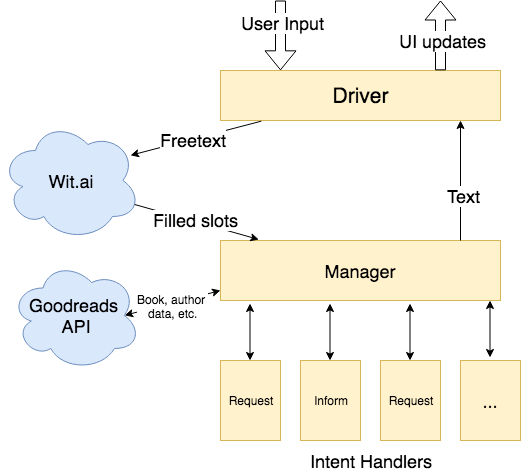
\includegraphics[scale=0.35]{architecture.jpg}
    \caption{A high-level architectural diagram of B. Rex.}
    \label{fig:arch}
\end{figure}

Figure \ref{fig:arch} provides an overview of how B. Rex's code is organized. Both a terminal interface for development and a web interface for deployment were created. Freetext user input was collected and sent to Wit.ai for NLU. Based on the value of the {\tt intent} slot returned by Wit.ai, the dialogue manager selects a handler, a section of code that is specifically written to handle that intent. For instance, the {\tt greet} handler is selected when the value of {\tt intent} is {\tt greet}, i.e. when Wit.ai detects that the user is attempting to greet B. Rex. The handler plans and generates its text output, which is then shown to the user.

\subsection{Wit.ai}\label{sec:witai}

Wit.ai is a platform that allows its users to take a pre-trained, general-purpose natural language understanding system and tailor it to their application domain by giving it training data. Because the model is pre-trained, the burden of producing training data is significantly reduced. In order to use Wit.ai with B. Rex, we had to decide on the slots we expected our user to fill (e.g. {\tt author}, {\tt genre}, etc.) and provide it with manually created and annotated utterances in order to teach it what utterances in our specific domain look like.

Using Wit.ai came with drawbacks that have to do with some inherent difficulties stemming from the unbounded nature of the domain of books. Unlike restaurants in a geographic area, there is an unlimited number of books, authors, and genres, so it is impossible for our training data to exhaustively cover ever possible value. We initially thought that context would be able to cue Wit.ai in on what kind of slot the sentence contained (e.g. ``I want a $[_{\mbox{\small genre}}$ literary fiction$]$ novel'' vs. ``I want a novel by $[_{\mbox{\small author}}$ Akhil Sharma$]$''). 
\begin{figure}
    \centering
    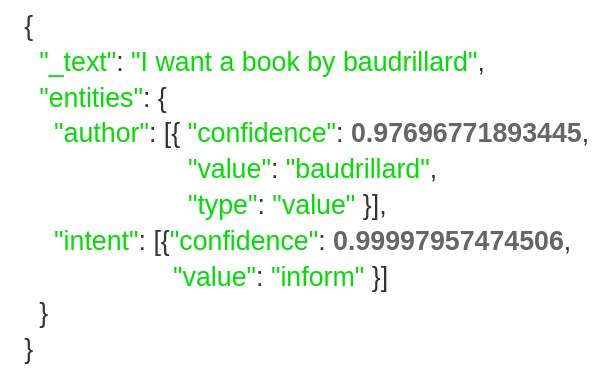
\includegraphics[scale=0.3]{witout.png}
    \caption{Sample JSON output from Wit.ai. {\tt \_text} contains the user's input, and {\tt entities} contains the slots Wit.ai found in the text, with their respective values.}
    \label{fig:without}
\end{figure}

Indeed, when we trained the system with expressions like this that contained more text than just what would fill the slot, Wit.ai mostly understood what the slot was supposed to be even when it had never encountered the value before. The issue, however, was that users almost always omitted this extra text, providing just the value of the slot, e.g. ``$[_{\mbox{\small ?}}$ literary fiction$]$''. In such circumstances, Wit.ai was usually not able to figure out which slot the value was intended for.  There is little that can be done to get around this problem unless an efficiently searchable database of genres, authors, and books is available and integrable into the NLU system. This would have taken a considerable amount of effort, so it was left out of scope.

\subsection{Handlers}

The handler that corresponds to the value of {\tt intent} is selected by the dialogue manager. Once the manager has selected the handler, it hands off all further execution to the handler, along with a few pieces of state: Wit.ai output, the entire history of the conversation, and conversational state shared across handlers. The handler then plans and generates a text response using this information as well as data retrieved from Goodreads on an as-needed basis. Finally, the text response is passed to the manager, which records the response as well as any changes in shared state made by the handler before passing the text to the user interface.  

We were satisfied with the way we designed the handler abstraction, as it allowed us to cleanly separate code that was specific to a certain behavior (e.g. recommending vs. providing information about a book). We found that handlers almost never needed to know about what other handlers were doing, and when they did, it was sufficient to put a few pieces of data in shared state.

\subsection{Goodreads}

We used a Python wrapper around the Goodreads API\footnote{{https://pypi.org/project/Goodreads/}} to retrieve information about authors, genres, books, etc. on Goodreads. Reviews had to be scraped manually with an XPath query, as they are not available through the Goodreads API.

A common user interaction is requesting more information about book that has been suggested. To fulfill these requests, we chose to take user reviews and use text summarization\footnote{We used sumy: {https://pypi.org/project/sumy/}} in order to ensure they would remain under a certain maximum length. (We found that 500 characters was the biggest screenful that was still small enough to be approachable.)

\subsection{Natural language generation}

We used Python string templates stored in files to generate our text. Every template is stored in a list that has a name corresponding to a certain system intent, such was {\tt summary} for when the system has decided that the user wants a summary of the selected book. A template is chosen randomly from the list for variety, and Python's {\tt format} function is used to fill the slots in the template.

\begin{figure}
    \centering
    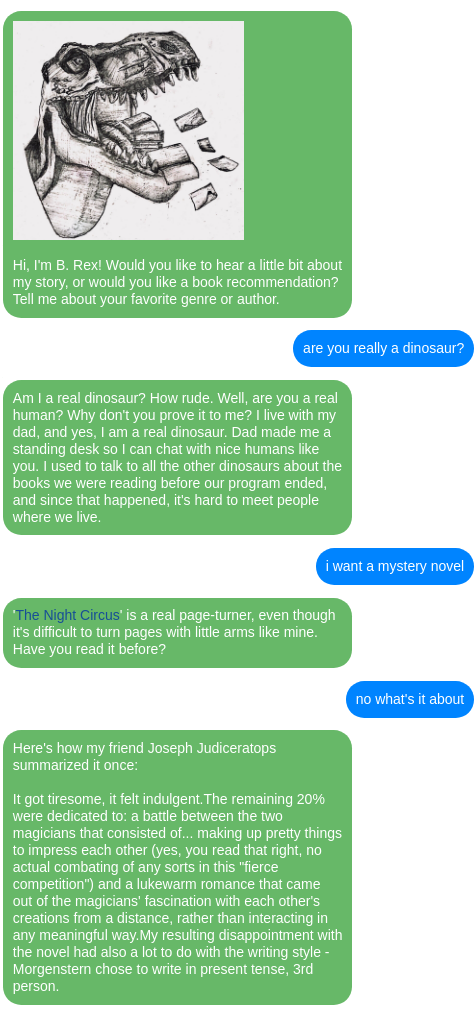
\includegraphics[scale=2.2]{sample.png}
    \caption{A sample dialogue with B. Rex.}
    \label{fig:sampledia}
\end{figure}

\subsection{B. Rex's persona}

A brief biosketch of B. Rex's life, personality, and preferences was written, and we referred to it as we wrote our template strings so that we could incorporate parts of B. Rex's persona into our responses and ensure that our attempts at developing his persona were specific enough to be believable and internally consistent. In addition to sprinkling in bits about his life into the task-oriented responses, we gave B. Rex the ability to talk directly about his favorite book, author, and genre. We followed the findings of \citeauthor{gilani:16} \shortcite{gilani:16} in having B. Rex respond as if he were \emph{really} a dinosaur behind a keyboard, instead of a virtual dinosaur created only for the purposes of this system.


\section{Evaluation}

\begin{figure*}
    \centering
    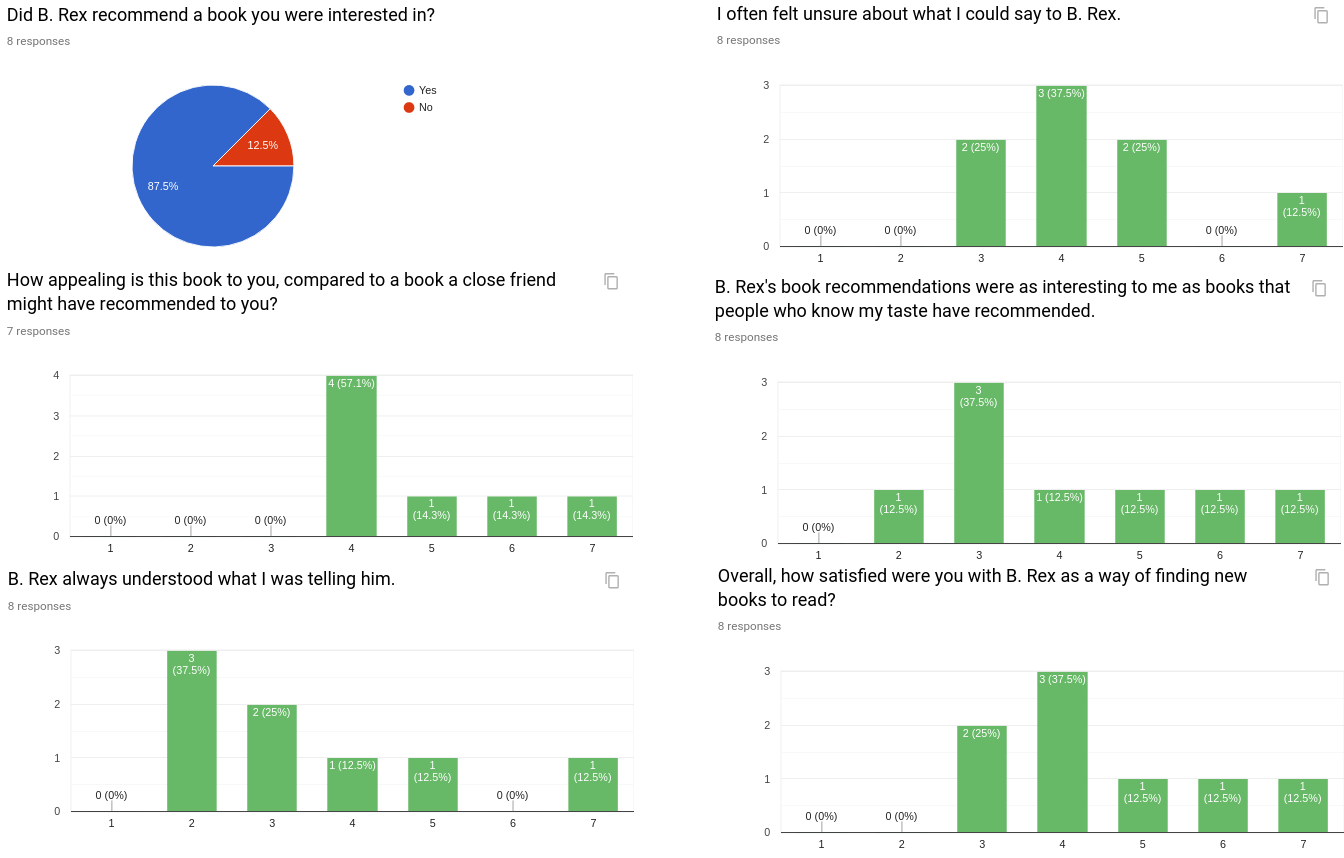
\includegraphics[scale=1.40]{results.png}
    \caption{Results of a survey given to B. Rex users. Freetext responses were also collected for the questions ``What was the worst part about talking to B. Rex?'', ``What was the best part about talking to B. Rex?", and ``Is there anything you expected B. Rex to do that he couldn't do?''.}
    \label{fig:results}
\end{figure*}

We evaluated our system with objective and subjective metrics collected from interactions with human users. We look particularly at task success, dialogue turns, and surveys in order to gain insight into the user experience. 

Similar to \citeauthor{Griol:13} \shortcite{Griol:13}, we gave a qualitative survey to discover strengths and weaknesses of our system. The questions we asked participants are given in figure \ref{fig:results} with their results. All participants were adults, so the extent to which these results generalize to children is unclear.

These results indicate that B. Rex was usually successful in recommending a book to users, indicating that users are succeeding in achieving a measure of successful communication with B. Rex. While some user feedback indicated that they had serious difficulties even getting a single book recommendation out of B. Rex, the bulk of user feedback about communication had to do with comparatively minor issues like the difficulty of Wit.ai not recognizing contextless slots in user input (described in section \ref{sec:witai}), or not recognizing certain genres or authors (a Goodreads problem). This trend in the freetext repsonses is supported by the scalar responses.

As for the quality of B. Rex's recommendations, according to the responses, it was for most users comparable to a slightly below average recommendation from a friend. Users liked the fact that they were offered another book if they rejected B. Rex's current suggestion. This level of quality seemed somewhat surprising given B. Rex's disadvantages compared to a book recommendation system like Amazon's or Goodreads's, since B. Rex only knows what the user has said, while Amazon and Goodreads have a better model of the user that has been constructed from much richer data sources. 

Our average number of turns to a first book recommendation was 3.28, and no dialogue that we recorded took longer than 8 turns to reach a first recommendation. 

In summary, it seems like the majority of user dissatisfaction had to do with poor understanding and relatively poor recommendation quality. These are both problems that could be easily solved by a commercial system with more training data and more user data, respectively\footnote{This comes with the caveat that identifying books and authors in isolation may remain somewhat difficult, as discussed in the introduction.}. As for successes, many of the users expressed their amusement with the B. Rex persona, and specifically mentioned a feature that invents an alliterative randomized fake reviewer name when B. Rex is presenting a review, e.g. ``Roger Rajasaurus''.

\section{Future work}

There are several immediate questions that would need to be addressed by extensions to this work.

First, the extent to which the system's performance generalizes to children is unclear, because all survey participants were adults. There may be characteristics of child dialogue that would make B. Rex perform better or worse. For example, if children were less likely to provide contextless slots (cf. section \ref{sec:witai}) than adults, B. Rex would perform better. On the other hand, if children made more spelling errors, B. Rex would probably perform worse. 

Second, there are many ways users want to discover books that are not possible at the moment. Users want to be able to find books that are similar to a certain book, that are by an author that is similar to a certain author, that were published within a certain year range, etc.

Third, an ideal book recommendation dialogue system must be able to answer high-level questions about a book. Users want to ask interpretive questions about books, like ``does it have a happy ending?'', ``does it have a major female character?'', etc. A fruitful way to tackle these questions would probably be to aggregate all user reviews for a book together and use methods from information retrieval and question answering systems to build a response.


\section{Conclusion}

In designing and creating B. Rex, we aimed to explore whether the process of book discovery could be made more accessible to some types of users who are less well served by the prevailing interfaces. We designed and implemented a dialogue system for book discovery that attempted to use a whimsical persona and the simplicity of the medium of dialogue in order to make the task of finding a book to read more simple and fun, which studies indicated would increase user engagement. Our system was able to successfully recommend books with acceptable quality to users, and users responded positively to the B. Rex persona.



% bibliography
\bibliography{naaclhlt2019}
\bibliographystyle{acl_natbib}



\end{document}

\end{document}


